\documentclass[conference]{IEEEtran}
\IEEEoverridecommandlockouts

\usepackage{graphicx}
\usepackage{booktabs}
\usepackage{tabularx}
\usepackage{array}
\usepackage{amsmath}
\usepackage{xcolor}
\usepackage{tikz}
\usepackage{pgfplots}
\pgfplotsset{compat=1.17}
\usetikzlibrary{positioning,arrows.meta,calc,fit,backgrounds,shapes.geometric}
\usepackage{fontspec}
\setmainfont{TeX Gyre Termes}
\setsansfont{TeX Gyre Heros}
\setmonofont{TeX Gyre Cursor}
\usepackage{xeCJK}
\setCJKmainfont{Noto Sans CJK JP}
\setCJKsansfont{Noto Sans CJK JP}
\setCJKmonofont{Noto Sans CJK JP}
\XeTeXlinebreaklocale "ja"
\XeTeXlinebreakskip=0pt plus 1pt
\usepackage{balance}
\usepackage[hidelinks]{hyperref}
\hypersetup{pdftitle={A Reference-Free Evaluation Funnel for Japanese News Summaries},
            pdfauthor={Chen Jinhua}}

\definecolor{navy}{HTML}{16233A}
\definecolor{cblue}{HTML}{2563EB}
\definecolor{cbluef}{HTML}{E7EEFD}
\definecolor{cgreen}{HTML}{15803D}
\definecolor{cgreenf}{HTML}{E7F5EB}
\definecolor{corange}{HTML}{C2620A}
\definecolor{corangef}{HTML}{FDF0E0}
\definecolor{cpurple}{HTML}{6D4AA8}
\definecolor{cpurplef}{HTML}{F0EBF9}
\definecolor{cred}{HTML}{B4211C}
\definecolor{credf}{HTML}{FBECEB}
\definecolor{cgray}{HTML}{5B6B7C}

\newcolumntype{Y}{>{\raggedright\arraybackslash}X}
\newcolumntype{R}{>{\raggedleft\arraybackslash}p{9mm}}
\renewcommand{\arraystretch}{1.05}
\setlength{\tabcolsep}{3.5pt}

\tikzset{
  stage/.style={rounded corners=1.6pt,draw=navy,line width=.35pt,fill=white,align=left,
                inner xsep=2.2mm,inner ysep=1.5mm,font=\sffamily\fontsize{6.4}{7.4}\selectfont},
  det/.style={stage,draw=cblue,fill=cbluef},
  emb/.style={stage,draw=cgreen,fill=cgreenf},
  sem/.style={stage,draw=corange,fill=corangef},
  scr/.style={stage,draw=cpurple,fill=cpurplef},
  term/.style={stage,draw=cred,fill=credf,text=cred,align=center},
  rev/.style={draw=navy,line width=.3pt,fill=white,rounded corners=6pt,align=center,
              inner xsep=1.6mm,inner ysep=.9mm,font=\sffamily\fontsize{5.8}{6.6}\selectfont},
  fl/.style={-{Stealth[length=1.5mm,width=1.1mm]},draw=cgray,line width=.4pt},
  kill/.style={-{Stealth[length=1.5mm,width=1.1mm]},draw=cred,line width=.4pt},
  cnt/.style={font=\sffamily\fontsize{5.8}{6.6}\selectfont,text=cgray},
  ttl/.style={font=\sffamily\fontsize{6.4}{7}\selectfont\bfseries}
}

\title{A Reference-Free Evaluation Funnel for Japanese News Summaries,\\
Delivered Twice as an Installable Plugin}

\author{\IEEEauthorblockN{Chen Jinhua}
\IEEEauthorblockA{AI Quality Scientist Take-Home Assignment\\
50 XL-Sum Japanese articles, 250 candidate summaries}}

\begin{document}
\maketitle

\begin{abstract}
A summariser in production is handed an article and returns a summary; nobody hands it a human reference. This report describes an evaluator built to that contract. Exploration showed the 250 supplied candidates are not a quality gradient but five distinct populations, and that the two most dangerous---fluent text that reverses the article, and fluent text that invents its central claim---are invisible to every cheap signal, because they are on topic by construction. The design separates constraints a script can prove from constraints only a reader can judge, and requires an independent reviewer to confirm every stopping decision. Validation rests on seven checks that do not share a failure mode, including a natural experiment in which the same candidate texts appear under both their own and a foreign article, and a third independent read of the 109 candidates for which no ground truth can be derived at all. The evaluator ships as an installable plugin, implemented twice on two agent hosts; the two implementations agree on routing for 94.4\,\% of candidates and on terminal category for 74 of 74.
\end{abstract}

\begin{IEEEkeywords}
LLM evaluation, reference-free metrics, summarisation quality, agent isolation, auditability, reproducibility
\end{IEEEkeywords}

\section{Exploration}

\subsection{First contact: what the 250 candidates actually are}
The dataset is 50 articles (483--3664 characters, median 1587) with a
human reference each (41--164 characters, median 93), and five opaque
candidates per article (22--302 characters, median 125).

Reading candidates side by side inside their articles, rather than as a
flat list, made the structure obvious within the first few articles: the
five candidates per article are not five samples from one generator.
They are draws from distinct populations. A string-level scan
of the corpus alone---no model, no scoring---confirmed and counted them
(Table~\ref{tab:census}). Four populations are mechanically derivable;
the fifth is the remainder and is the interesting one.

\begin{table}[t]
\caption{Corpus census. Categories derived from the corpus by string
comparison only, with no evaluator output involved. Used at the very end
as weak labels, never during scoring.}
\label{tab:census}
\centering\footnotesize
\begin{tabularx}{\columnwidth}{@{}p{27mm}rY@{}}
\toprule
\textbf{Population} & \textbf{$n$} & \textbf{Derivation} \\
\midrule
Reference reproduced   & 58  & candidate $=$ reference \\
Copy of the article    & 50  & candidate $\subset$ article body \\
Reference fragment     & 17  & reference starts with candidate \\
Belongs elsewhere      & 16  & matches a \emph{different} article \\
Generated, unlabelled  & 109 & none of the above \\
\midrule
\textbf{Total}         & \textbf{250} & \\
\bottomrule
\end{tabularx}
\end{table}

Three structural facts came out of the same scan and shaped everything
downstream.

\emph{The sentence limit is almost never the problem.} Only three of 250
candidates exceed three sentences, and all three are article copies that
would be stopped anyway. A rule that enforces the stated product
specification is necessary but will almost never fire; treating
``$\leq 3$ sentences'' as the headline quality dimension would have been
a serious misallocation of effort.

\emph{The corpus contains an accidental controlled experiment.} Twenty
groups of candidates share byte-identical text after Unicode
normalisation. Eight of those groups sit inside a single article---the
same text scored twice, independently. Fourteen span articles: the same
text is attached to its own article in one place and to a foreign
article in another. This is a free reliability instrument and Section~III
uses it as one.

\emph{The references are not ground truth, and the data says so.} The
assignment warns that XL-Sum reference quality is uneven. It is worse
than uneven: several references assert facts the article body never
contains. The reference for article \texttt{35278497} states a 4割
sexual-assault share, a suspect profile, and a 379-case figure, none of
which appear in the supplied text; the reference for
\texttt{features-and-analysis-46643494} is a photo caption that opens
with \mbox{この写真}, a demonstrative whose antecedent exists only in an image
nobody is given. Any design that scores a candidate by its distance to
the reference would reward reproducing these.

\subsection{Hypotheses, and which ones died}
Five hypotheses were formed before building anything. Two survived
unchanged, one survived in weakened form, and two were killed by the
data (Table~\ref{tab:hyp}).

\begin{table}[t]
\caption{Hypotheses formed during exploration and their fate.}
\label{tab:hyp}
\centering\footnotesize
\begin{tabularx}{\columnwidth}{@{}>{\raggedright\arraybackslash\hyphenpenalty=10000\exhyphenpenalty=10000}p{31mm}Y@{}}
\toprule
\textbf{Hypothesis} & \textbf{Outcome} \\
\midrule
Copying is detectable with string evidence, not embeddings &
\textbf{Survived.} A copy is maximally similar to its article, so
similarity is exactly the wrong instrument. Containment and $n$-gram
coverage caught 50 of 50. \\
\addlinespace[1pt]
Embedding similarity separates topic mismatch &
\textbf{Survived.} Two disjoint 10-article probes: matched 0.707--0.868,
mismatched 0.163--0.398. \\
\addlinespace[1pt]
Similarity can screen relevance on its own &
\textbf{Weakened.} On all 250 pairs the bands overlap: off-topic reaches
0.4813, on-topic falls to 0.4034. It may nominate; it may not decide. \\
\addlinespace[1pt]
Missing sentence-final punctuation indicates truncation &
\textbf{Killed.} \mbox{体言止め}---a verbal noun closing a headline---is
standard Japanese news register and looks identical to an amputated
predicate. \\
\addlinespace[1pt]
Factual defects form one gradient, so one faithfulness score suffices &
\textbf{Killed.} A wrong peripheral number and a reversed main event are
not two points on a scale; one is a flawed summary, the other is a
false one. \\
\bottomrule
\end{tabularx}
\end{table}

The last row is the finding the rest of the design turns on. Inspecting
the 109 unlabelled candidates one by one exposed a failure mode with no
detector anywhere in the pipeline as it then stood: text that is fluent,
within the sentence limit, not a copy, not truncated, on topic, and
\emph{states the opposite of the article}. Article \texttt{41396293}
reports the Japanese prime minister announcing a dissolution of the
lower house; its candidate \texttt{0c954428} reports him announcing that
he will \emph{not} dissolve it. Article \texttt{34991666} reports two
attackers dead; candidate \texttt{f6f8e339} reports them fled to another
state and still at large. Nothing upstream can see this. The string
evidence is clean. The embedding similarity is \emph{high}, because the
topic is right---that is precisely why the failure is dangerous. A
sibling mode invents rather than inverts: candidate
\texttt{41875333\_aa36a21a} attributes to the US president the quoted
line 「米国はもはや世界の警察ではない」, which appears nowhere in the
article and displaces the claim the headline actually makes.

Set against these, a case such as \texttt{40490051\_5d9feeef} is a
different animal: it substitutes five details (シリア for イラク,
男性 for 女性, 30代 for 10代, 8000 for 6000, 500 for 300) while the
central event---a fierce IS-clearing battle in Mosul's old city---is
correctly reported. It is a bad summary, not a false one, and an
evaluation that collapses both into ``score zero'' has thrown away the
ranking the application needs.

\section{Design}

\subsection{The evidence boundary}
The runtime evaluator sees exactly one article and one candidate---never
a reference, never another article, never a corpus. This is not a
stylistic preference: a signal that needs a second article is
unavailable to a caller who sent one request, and a signal derived from
a reference is unavailable to an application whose purpose is to run
where no reference exists. An earlier relevance gate ranked each
candidate against every article in the batch; that evidence was removed
even though it worked, because it measured something the deployed system
cannot. References enter once, after every score is final, in
Section~III.

\subsection{Two layers of hard constraint, then a graded score}
Figure~\ref{fig:funnel} is the funnel, annotated with the actual counts
from the submitted run. The organising principle is that constraints
divide by what kind of evidence can settle them.

\emph{Layer~1 is physical.} Empty output, sentence count above three,
and near-verbatim copying are settled by a script, because the
measurement \emph{is} the conclusion: a containment ratio near 1.0 is
not evidence of copying, it is copying.

\emph{Layer~2 is semantic.} Whether a candidate is grounded in its
article cannot be settled by any measurement, so a dedicated Grounding
Gate agent screens every survivor before any scoring happens. It answers
one question---is this candidate grounded?---and returns at most one
central category (\textsc{off\_topic}, \textsc{factual\_reversal},
\textsc{fabricated\_content}) with one article span and one candidate
span as evidence. It is deliberately blind to quality: it never receives
the rubric, never sees the anchor, and cannot emit a score. An agent
that both screens and scores will trade a central defect for a low
score instead of stopping it.

Between the two layers sits embedding relevance, which is
\emph{required but never terminal}. Every survivor must leave that stage
carrying a similarity value against its own article; a run that could
not reach the embedding model is incomplete, not cheaper. But a value
below threshold is only a hint that the semantic layer should look
closely.

Survivors of both layers receive a graded score
(Table~\ref{tab:rubric}). Weights follow directly from the exploration:
faithfulness carries half the total because fluent-but-false is the
dominant risk in this corpus, and conciseness carries five points
because the sentence limit is already a hard constraint and almost never
violated.

\begin{table}[t]
\caption{Soft rubric. Applied only to candidates that survive both hard
layers. The four dimensions sum to the total exactly.}
\label{tab:rubric}
\centering\footnotesize
\begin{tabularx}{\columnwidth}{@{}p{18mm}rYr@{}}
\toprule
\textbf{Dimension} & \textbf{Max} & \textbf{Question} & \textbf{Mean} \\
\midrule
Faithfulness & 50 & Is every claim supported by the article? & 38.7 \\
Coverage     & 30 & Is the main event and its key facts present? & 19.0 \\
Coherence    & 15 & Complete, grammatical, ordered? & 13.5 \\
Conciseness  &  5 & Compact, without repetition? & 4.8 \\
\midrule
\textbf{Total} & \textbf{100} & \multicolumn{2}{r}{\textbf{76.1} over 165 survivors} \\
\bottomrule
\end{tabularx}
\end{table}

Terminal outcomes all score 0 but keep separate rank tiers, so five
candidates remain orderable even when several fail. Reversal,
fabrication and off-topic share the worst tier, because each misleads a
reader who cannot check the source; copying and truncation rank above
them, because a copy at least contains true sentences.

\subsection{Independent review of every stopping decision}
No stage in the funnel may stop a candidate on its own authority. Each
proposal---from the script, from the grounding gate, from the scorer's
backstop---goes to a Reviewer in a fresh context that re-derives the
evidence from the article. The review is not a rubber stamp: in the
submitted run it rejected 2 of 53 physical proposals, 8 of 37 grounding
proposals (including all eight fabrication claims), and 3 of 4 late
scorer proposals, sending each rejected case onward to be scored rather
than stopped. It also escalated four truncations the gate had not
proposed. Disagreement that survives one revision round is preserved as
low confidence rather than averaged away.

\begin{figure}[t]
\centering
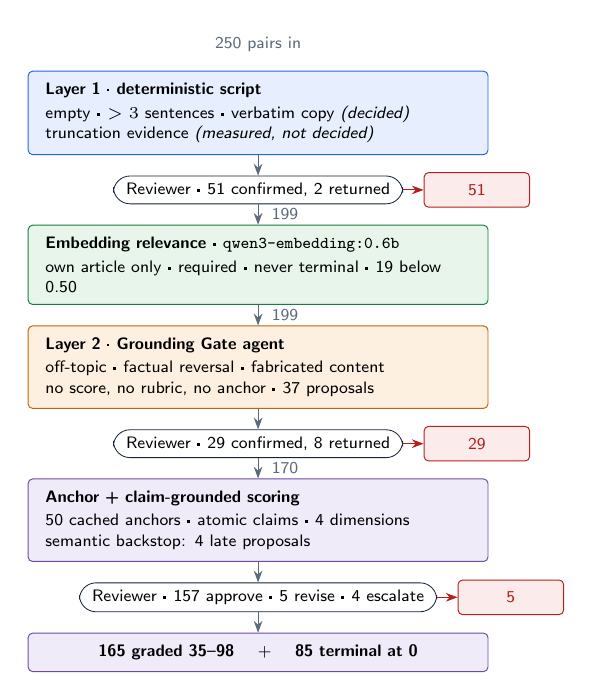
\begin{tikzpicture}[node distance=0mm]
\node[det,text width=54mm] (s1) {%
  \textbf{Layer 1 · deterministic script}\\[.4mm]
  empty · $>3$ sentences · verbatim copy \emph{(decided)}\\
  truncation evidence \emph{(measured, not decided)}};
\node[rev,below=2.6mm of s1] (r1) {Reviewer · 51 confirmed, 2 returned};
\node[emb,below=2.6mm of r1,text width=54mm] (s2) {%
  \textbf{Embedding relevance} · \texttt{qwen3-embedding:0.6b}\\[.4mm]
  own article only · required · never terminal · 19 below 0.50};
\node[sem,below=2.6mm of s2,text width=54mm] (s3) {%
  \textbf{Layer 2 · Grounding Gate agent}\\[.4mm]
  off-topic · factual reversal · fabricated content\\
  no score, no rubric, no anchor · 37 proposals};
\node[rev,below=2.6mm of s3] (r2) {Reviewer · 29 confirmed, 8 returned};
\node[scr,below=2.6mm of r2,text width=54mm] (s4) {%
  \textbf{Anchor + claim-grounded scoring}\\[.4mm]
  50 cached anchors · atomic claims · 4 dimensions\\
  semantic backstop: 4 late proposals};
\node[rev,below=2.6mm of s4] (r3) {Reviewer · 157 approve · 5 revise · 4 escalate};
\node[scr,below=2.6mm of r3,text width=54mm,align=center] (out) {%
  \textbf{165 graded 35--98} \quad + \quad \textbf{85 terminal at 0}};

\node[cnt,above=1.2mm of s1] {250 pairs in};
\coordinate (rt) at ($(s1.east)+(4.2mm,0)$);
\node[term,right=2.6mm of r1.east,yshift=0mm,text width=9mm] (t1) {51};
\node[term,right=2.6mm of r2.east,text width=9mm] (t2) {29};
\node[term,right=2.6mm of r3.east,text width=9mm] (t3) {5};

\draw[fl] (s1) -- (r1);
\draw[fl] (r1) -- node[cnt,right=0.5mm]{199} (s2);
\draw[fl] (s2) -- node[cnt,right=0.5mm]{199} (s3);
\draw[fl] (s3) -- (r2);
\draw[fl] (r2) -- node[cnt,right=0.5mm]{170} (s4);
\draw[fl] (s4) -- (r3);
\draw[fl] (r3) -- (out);
\draw[kill] (r1.east) -- (t1.west);
\draw[kill] (r2.east) -- (t2.west);
\draw[kill] (r3.east) -- (t3.west);
\end{tikzpicture}
\caption{The funnel, annotated with counts from the submitted 250-pair
run. Red exits are Reviewer-confirmed terminations. The 51 pairs
stopped at layer~1 cost one script pass and one confirmation; 80 of 250
never reach anchor generation and scoring, the most expensive stage.}
\label{fig:funnel}
\end{figure}

\subsection{Alternatives considered and rejected}
Table~\ref{tab:rejected} lists the approaches that were tried and
dropped, each with the measurement that killed it. Two deserve a
sentence. A cross-encoder reranker
(\texttt{bge-reranker-v2-m3}) separates the off-topic population more
cleanly than the embedding does in mean terms---0.0001 against
0.9300---but at a 0.50 cut it flags 15 legitimate candidates as
unrelated where the embedding flags 3, so it buys no recall and costs
five times the false alarms. And embedding the candidate against the
generated anchor correlated better with coverage
($\rho = 0.630$ versus $0.528$) yet predicted it worse under
leave-one-out (MAE 4.01 versus 3.62); a feature that correlates better
and predicts worse is a feature fitted to the sample, so the anchor
stayed a reasoning aid and never became a number.

\begin{table}[t]
\caption{Rejected approaches and the evidence that rejected them.}
\label{tab:rejected}
\centering\footnotesize
\begin{tabularx}{\columnwidth}{@{}>{\raggedright\arraybackslash\hyphenpenalty=10000}p{25mm}Y@{}}
\toprule
\textbf{Approach} & \textbf{Why it was rejected} \\
\midrule
Score against the reference &
Unavailable in production, and demonstrably wrong here: 45 of 50
references were outscored by a generated candidate in their own
article. \\
\addlinespace[1pt]
Similarity as a quality score &
A verbatim copy is the most similar text there is. \\
\addlinespace[1pt]
Cross-encoder reranker &
Same recall (16/16), five times the false positives (15 vs.\ 3 of 234)
at a 0.50 cut. \\
\addlinespace[1pt]
Anchor similarity as a scoring feature &
Higher correlation, worse leave-one-out error. \\
\addlinespace[1pt]
Batch-relative relevance &
Uses articles a production caller never sent. Removing it changed
0 of 19 nominations. \\
\addlinespace[1pt]
Regex decides truncation &
\mbox{体言止め} is indistinguishable from an amputated predicate without the
deleted text. \\
\addlinespace[1pt]
One agent screens \emph{and} scores &
It trades a central defect for a low score instead of stopping. \\
\bottomrule
\end{tabularx}
\end{table}

\subsection{Delivery: the design is a plugin, not a script}
The evaluator is packaged as an installable plugin so that anyone who
needs it can run it rather than reconstruct it. The primary
implementation is a Claude Code plugin: one slash command, one skill,
four isolated agents (Grounding Gate, Scorer, Reviewer, Reporter) and
the deterministic scripts they call. Installation is two commands
against a local marketplace declared in the repository. There is no
orchestration notebook, no prompt to paste and no hidden state---the
manifest, rubric, few-shot bank and agent contracts are all files under
version control, so a reviewer can read exactly what each role was
told.

The same design is implemented a second time as a Codex plugin. This is
not redundancy for its own sake---it is the instrument for the
cross-host check in Section~III-F. Both plugins emit the same record
schema, including an \texttt{evaluation\_trace} that lists every stage
visited with its evidence, so any score in \texttt{scores.jsonl} can be
replayed backwards to the measurement that produced it.

\section{Validation}

An evaluation is only worth its weakest justification, so the goal here
was several checks that fail differently rather than one check repeated.
Table~\ref{tab:val} is the summary; the subsections give the reasoning.

\begin{table}[t]
\caption{Seven validation checks on the submitted run. ``A'' is the
primary Claude-plugin run, ``B'' the independent Codex-plugin run.}
\label{tab:val}
\centering\footnotesize
\begin{tabularx}{\columnwidth}{@{}>{\raggedright\arraybackslash\hyphenpenalty=10000}p{24mm}Yr@{}}
\toprule
\textbf{Check} & \textbf{What it tests} & \textbf{Result} \\
\midrule
Arithmetic \& bands & 500 records, sums and label boundaries & 0 errors \\
Repeated text & 8 duplicate pairs inside one article & 8/8, 8/8 \\
Pair conditioning & 14 texts under own \emph{and} foreign article & 14/14, 14/14 \\
Weak labels & 141 corpus-derivable categories & .915 / .901 \\
Within-article order & planted failure vs.\ its reference & 0/50, 0/50 \\
Cross-host routing & A vs.\ B on 250 pairs & .944 \\
Third read & 109 candidates with no ground truth & $\rho$ .960 \\
\bottomrule
\end{tabularx}
\end{table}

\subsection{Internal consistency}
Across the 500 records of both runs, every soft score equals the sum of
its four dimensions and every quality label falls inside its declared
band; there are zero arithmetic and zero banding violations. This is a
floor, not a result---it says the machinery did what it claims, nothing
about whether the judgements are right.

\subsection{The same text, scored twice}
Eight groups of candidates are byte-identical \emph{and} attached to the
same article. Each was scored independently, in a separate context,
without either scorer knowing the twin existed. All eight received
identical totals \emph{and} identical values on all four dimensions, in
both implementations. Run-to-run variance on repeated input is
therefore not the reason for any spread reported below.

\subsection{A natural experiment in pair conditioning}
Fourteen further groups are byte-identical but split across articles:
the same text sits under its own article in one place and under a
foreign one in another. If the evaluator were grading text quality, it
would give both copies the same score. It does not. In all 14 groups,
in both implementations, the foreign placement was terminated at 0 as
off-topic and the native placement was graded on its merits---for
instance the text of \texttt{54083932\_9e7163bb} scores 87 under its own
article and 0 as \texttt{44708203\_6d931562} under another. The
evaluator is conditioning on the pair, which is what the contract
requires and what a text-only metric cannot do.

\subsection{Agreement with corpus-derived weak labels}
After both runs were final, references were opened for the first time
and the Table~\ref{tab:census} categories were used as weak labels.
Figure~\ref{fig:bands} shows the outcome distribution per population.
All 50 article copies and all 16 foreign-article candidates terminated,
in both runs. No reference reproduction was ever terminated. Overall
agreement on the 141 labellable candidates is 129/141 ($0.915$) for run
A and 127/141 ($0.901$) for run B.

Two things in that figure matter more than the headline number. First,
the fragment population is graded rather than uniformly stopped: 5 of 17
terminate and the remaining 12 land between 39 and 70, none reaching
\textsc{good}. That is a deliberate divergence from the label, discussed
in Section~IV, not a detection failure. Second, \emph{no} reference
reproduction reached \textsc{excellent} while 28 generated candidates
did. This is the reference-quality problem made quantitative: the
evaluator credits only what the article body supports, and XL-Sum
references routinely assert more than that.

\begin{figure}[t]
\centering
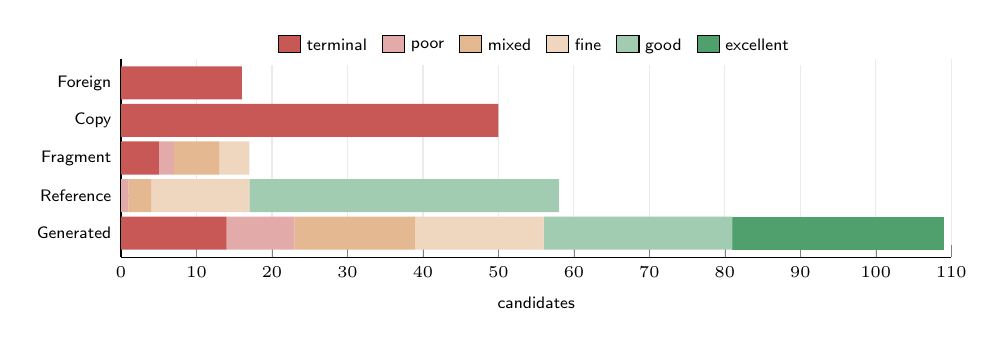
\begin{tikzpicture}
\begin{axis}[
  width=\columnwidth, height=41mm,
  xbar stacked, xmin=0, xmax=110,
  bar width=4.2mm,
  ytick=data,
  symbolic y coords={Foreign,Copy,Fragment,Reference,Generated},
  y dir=reverse,
  tick label style={font=\sffamily\fontsize{6}{7}\selectfont},
  label style={font=\sffamily\fontsize{6.4}{7.4}\selectfont},
  xlabel={candidates},
  legend style={font=\sffamily\fontsize{5.6}{6.4}\selectfont,
                at={(0.5,1.16)},anchor=north,legend columns=6,
                draw=none,/tikz/every even column/.append style={column sep=1.2mm}},
  axis lines*=left, x tick label style={/pgf/number format/fixed},
  xmajorgrids, grid style={draw=black!8},
  enlarge y limits=0.16,
]
\addplot[fill=cred!75,draw=none] coordinates {(16,Foreign) (50,Copy) (5,Fragment) (0,Reference) (14,Generated)};
\addplot[fill=cred!38,draw=none] coordinates {(0,Foreign) (0,Copy) (2,Fragment) (1,Reference) (9,Generated)};
\addplot[fill=corange!45,draw=none] coordinates {(0,Foreign) (0,Copy) (6,Fragment) (3,Reference) (16,Generated)};
\addplot[fill=corange!26,draw=none] coordinates {(0,Foreign) (0,Copy) (4,Fragment) (13,Reference) (17,Generated)};
\addplot[fill=cgreen!40,draw=none] coordinates {(0,Foreign) (0,Copy) (0,Fragment) (41,Reference) (25,Generated)};
\addplot[fill=cgreen!75,draw=none] coordinates {(0,Foreign) (0,Copy) (0,Fragment) (0,Reference) (28,Generated)};
\legend{terminal,poor,mixed,fine,good,excellent}
\end{axis}
\end{tikzpicture}
\caption{Outcome of the primary run by corpus-derived population. The
two populations that should never survive never do; the fragment
population is graded rather than stopped; and no reference reproduction
reaches the top band.}
\label{fig:bands}
\end{figure}

\subsection{Within-article ordering}
The application needs candidates ordered inside an article, so ordering
was checked directly rather than inferred from scores. Across all 50
articles, in both runs, \emph{zero} articles placed a planted failure at
or above the reference reproduction for that article. Ordering is also
not degenerate: the median spread between the best and worst surviving
candidate within an article is 26 points (maximum 61), and every article
retained between two and four survivors, so no article was either wiped
out or passed untouched.

\subsection{Two implementations, two hosts}
The strongest available check on a design---as opposed to a run---is to
implement it twice and compare. The Codex plugin was written against the
same rubric but a different host, different agent runtime and different
underlying model, and neither implementation saw the other's output.

On 250 pairs the two agree on routing (terminal versus graded) for 236,
or $94.4\,\%$, and on \emph{which} terminal category, for all 74 pairs
both stopped. On the 162 pairs both graded, Spearman
$\rho = 0.891$ with a mean absolute difference of 6.85 points and a
signed mean of $-1.97$ (Fig.~\ref{fig:xhost}).

The disagreements are more informative than the agreements, and they are
one-sided in a way that is easy to explain. All 11 pairs stopped only by
A are severity calls on a defect B also found: 6 reversals, 4 fragments
and 1 fabrication, which B scored between 28 and 66---low, but not
stopped. The 3 stopped only by B were scored 58--71 by A. Not one
disagreement is a case where one implementation saw a defect the other
missed entirely. The two systems disagree about where the cliff is, not
about which candidates are near it.

Exact agreement on the five-band label is only 88 of 162 ($54.3\,\%$),
and that number is reported here because it is the least flattering
result in the report. It is a banding artefact---a mean absolute
difference of 6.85 straddles boundaries that are 10 to 15 points
wide---but it is a real caution: the bands are convenient for a reader
and should not be treated as stable, whereas the underlying ordering is.

\begin{figure}[t]
\centering
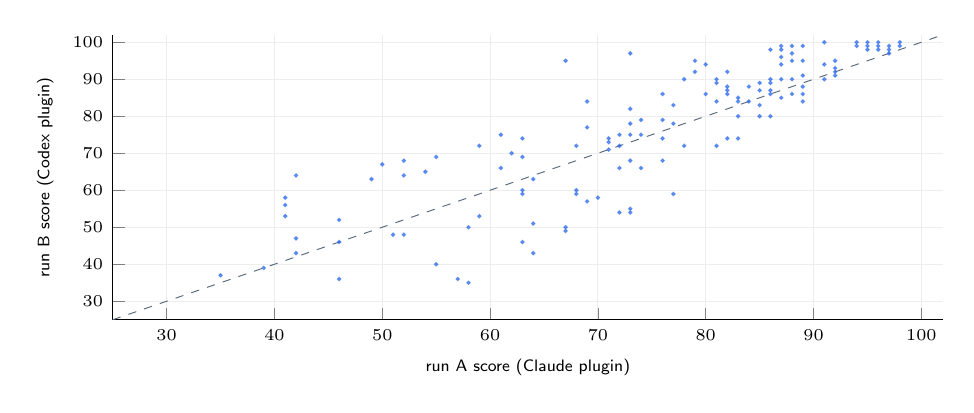
\begin{tikzpicture}
\begin{axis}[
  width=\columnwidth, height=52mm,
  xmin=25,xmax=102,ymin=25,ymax=102,
  xlabel={run A score (Claude plugin)},
  ylabel={run B score (Codex plugin)},
  tick label style={font=\sffamily\fontsize{6}{7}\selectfont},
  label style={font=\sffamily\fontsize{6.4}{7.4}\selectfont},
  xtick={30,40,50,60,70,80,90,100},
  ytick={30,40,50,60,70,80,90,100},
  grid=both, grid style={draw=black!7},
  axis lines*=left,
]
\addplot[only marks,mark=*,mark size=.6pt,draw=cblue,fill=cblue,opacity=.6] coordinates {
(35,37) (39,39) (41,53) (41,56) (41,58) (42,43) (42,47) (42,64) (46,36) (46,46)
(46,52) (49,63) (50,67) (51,48) (52,48) (52,64) (52,68) (54,65) (55,40) (55,69)
(57,36) (58,35) (58,50) (59,53) (59,72) (61,66) (61,75) (62,70) (63,46) (63,59)
(63,60) (63,69) (63,74) (64,43) (64,51) (64,63) (67,49) (67,50) (67,95) (68,59)
(68,60) (68,72) (69,57) (69,77) (69,84) (70,58) (71,71) (71,73) (71,74) (72,54)
(72,66) (72,72) (72,75) (73,54) (73,55) (73,68) (73,75) (73,78) (73,82) (73,97)
(74,66) (74,75) (74,79) (76,68) (76,74) (76,79) (76,86) (77,59) (77,78) (77,83)
(78,72) (78,90) (79,92) (79,95) (80,86) (80,94) (81,72) (81,84) (81,89) (81,90)
(82,74) (82,86) (82,87) (82,88) (82,92) (83,74) (83,80) (83,84) (83,85) (84,84)
(84,88) (85,80) (85,83) (85,87) (85,89) (86,80) (86,86) (86,87) (86,89) (86,90)
(86,98) (87,85) (87,90) (87,94) (87,96) (87,98) (87,99) (88,86) (88,90) (88,95)
(88,97) (88,99) (89,84) (89,86) (89,88) (89,91) (89,95) (89,99) (91,90) (91,94)
(91,100) (92,91) (92,92) (92,93) (92,95) (94,99) (94,100) (95,98) (95,99) (95,100)
(96,98) (96,99) (96,100) (97,97) (97,98) (97,99) (98,99) (98,100)};
\addplot[draw=cgray,dashed,line width=.35pt,forget plot] coordinates {(25,25) (102,102)};
\end{axis}
\end{tikzpicture}
\caption{The 162 candidates graded by both implementations.
$\rho = 0.891$, mean absolute difference 6.85 points. The dashed line is
equality.}
\label{fig:xhost}
\end{figure}

\subsection{The block with no ground truth}
Every check so far rests on the 141 candidates the corpus can label. But
those are the easy ones: copies, fragments and misfiled text are
detectable by construction. The 109 generated candidates---the block
that actually carries the fluent factual errors---have no derivable
label at all, and they are 44\,\% of the corpus. An evaluation that
reports 0.915 agreement while remaining silent about this block is
reporting the wrong number.

So the 109 were scored a third time, by a separate reading that used the
same rubric but had no access to either run's output. Against the
primary run this third read gives $\rho = 0.960$ with a mean absolute
difference of 4.09 points; against the secondary run,
$\rho = 0.936$ and 5.95 points. More pointedly: the 14 candidates the
primary run terminated in this block were given a mean of 32.5 by the
independent read (range 20--53) against 77.0 for the rest. An
independent reader who was never told those candidates had been stopped
put every one of them at the bottom of the distribution.

This does not make the scores correct---three readings of the same
rubric can share a bias, and none of them is a human judgement. What it
does establish is that the signal on the unlabelled block is
reproducible rather than idiosyncratic, which is the claim that was
actually missing.

\subsection{Reproducing the numbers in this report}
Every quantity quoted above is re-derived from the shipped artifacts by
\texttt{code/valid\-ation/verify\_report\_numbers.py}, which reads only
\texttt{data/}, the two run files and the third-read file, and asserts
each claim. It prints 91 checks and exits non-zero if any of them moves.
A reader who does not trust a number in this report can recompute it in
one command rather than take it on faith.

\section{Limitations}

\subsection{What the evaluation does not measure}
No human judgement enters anywhere. Every agreement number in
Section~III is either agreement with a mechanically derived label or
agreement between readings of the same rubric, and neither is accuracy.
The honest ceiling on all of it is \emph{reproducible}, not
\emph{correct}.

Reference reproductions are treated as acceptable by the weak-label
check, which Section~I showed is not safe: the worst of them scores 42
and the evaluator was right to say so. The label and the evaluator
disagree there, and the label is wrong.

It also measures nothing a reader would call style, register or audience
fit: beyond grammatical completeness it has no view on whether a summary
is well written, nor on the newsworthiness of the facts chosen---only on
whether they are the article's main ones.

\subsection{What it measures poorly}
Truncation is the weak point, and the failure is partly structural. A
one-record probe made this concrete: candidate
\texttt{51395937\_e409196f} is the reference cut from 「…\mbox{方針を\mbox{発表}}した。」
to 「…\mbox{方針を\mbox{発表}}」. The Reviewer declined to call it truncated, arguing
that \mbox{発表} is a verbal noun discharging the clause and that this is
ordinary headline register. The argument is sound and the conclusion is
wrong---the corpus shows the deleted characters were した。 Nothing in
the article or the candidate distinguishes \mbox{体言止め} from an amputated
predicate; only the deleted text does, and a reference-free evaluator
does not have it. The fragment population therefore splits in two:
endings amputated mid-token (\mbox{しかしそ}, \mbox{女性2人が車}, \mbox{救助し}) are visible
and missing them is a recall problem worth fixing, while \mbox{体言止め} endings
are undecidable under the contract and should not be counted against the
evaluator. Reporting both as one category, as the 5-of-17 figure does,
overstates the deficiency.

The five-band labels are less stable than the scores, as
Section~III-F showed. Bands are for readers; ordering is for decisions.

Cost is uneven. The funnel settles 51 of 250 pairs with a script and one
confirmation pass and keeps 80 of 250 out of anchor generation and
scoring entirely, but the price of moving the truncation judgement from
the script to the Reviewer is that a fragment now consumes both before
it is stopped---about six percent of the scoring work in this run.

\subsection{One structural gap, stated plainly}
The Reviewer in the submitted run held file-read tools and the corpus
sat on disk with its reference column intact. Its inputs contained no
reference field and the artifacts show none was used, but that is a
guarantee by convention, and a convention is not evidence. A
structurally blind Reviewer that receives article and candidate inline
and holds no read tools is written and shipped in both plugins; no run
has used it yet. The right next step is to re-adjudicate the 85 terminal
decisions with it and publish the delta, because that number is the
honest measure of how much the reachability of a reference mattered.

\subsection{What I would do next}
More data, first and above everything else. The whole report rests on
250 pairs from 50 articles of one publisher in one language, with a
median article length of 1587 characters. Every threshold here---the
0.50 similarity cut, the four dimension maxima, the five band
boundaries---is calibrated to that sample and should be assumed invalid
outside it. The immediate work is to run the same funnel over a much
larger Japanese corpus drawn from several publishers, then across
languages, because a design whose hard constraints include Japanese
sentence segmentation and \mbox{体言止め} register has obvious
language-specific parts that must be re-derived rather than translated.
Only after that does it make sense to spend on human adjudication of a
stratified sample, controlled perturbations for numbers, entities,
negation and causality, and re-calibration of the embedding threshold
per model and domain.

\section{Conclusion}
This is a working, fully audited prototype with evidence on one corpus:
250 pairs routed, 85 stopped by a confirmed terminal decision, 165
graded between 35 and 98, no arithmetic error, no ordering inversion
against a reference, 94.4\,\% routing agreement with an independently
implemented twin, and a reproducible signal on the 44\,\% of the corpus
where no ground truth exists. It is not a production accuracy guarantee,
for the reason in Section~IV-D: one corpus, one language, one publisher.
What the design provides is the property that makes the next corpus
cheap---it installs as a plugin, and every score carries the trace that
produced it.

\balance
\end{document}
